%\documentclass[conference]{IEEEtran}
\documentclass[12pt,journal,draftcls,doublespace, letterpaper,onecolumn]{IEEEtran}
\IEEEoverridecommandlockouts
% The preceding line is only needed to identify funding in the first footnote. If that is unneeded, please comment it out.
\usepackage{cite}
\usepackage{amsmath,amssymb,amsfonts}

\usepackage{algorithm}  
\usepackage{algpseudocode}  
\usepackage{amsmath}  
\renewcommand{\algorithmicrequire}{\textbf{Input:}}  % Use Input in the format of Algorithm  
\renewcommand{\algorithmicensure}{\textbf{Output:}} % Use Output in the format of Algorithm  
\usepackage{graphicx}
\usepackage{textcomp}
\usepackage{xcolor}
\usepackage{pythonhighlight}
\def\BibTeX{{\rm B\kern-.05em{\sc i\kern-.025em b}\kern-.08em
    T\kern-.1667em\lower.7ex\hbox{E}\kern-.125emX}}

\newtheorem{theorem}{Theorem}
\newtheorem{lemma}{Lemma}
\newtheorem{corollary}{Corollary}
\newtheorem{defn}{Definition}[section]

\begin{document}

\title{The characterization of attack patterns from 
	comprehensive, multi-source cyber-security events\\
}

\author{\IEEEauthorblockN{1\textsuperscript{st} Yuting Zhang}
\IEEEauthorblockA{\textit{Department of Information Security, Zhejiang University, Hangzhou, China} \\
Hangzhou, China \\
zjuzyting@gmail.com}
}


\maketitle

\begin{abstract}
	Based on data analysis, dimension reduction clustering, feature matching and other algorithms, this paper studies the characteristics of attack events in multi-source network flow events. We start with a systematic definition of attack events and attack patterns and explain the implications of data in multi-source network flows. Secondly, we combined the data of different dimensions and the data defined as attack events to extract the features of attack events in different dimensions. Here, we used the excellent t-sne dimensionality reduction algorithm and the mixed gaussian model to classify and extract the features. A variety of attack patterns can be obtained by reclassifying attack events according to attack characteristics, and data that may become attack events can be obtained by matching attack patterns with original data. With the above method, the identification accuracy rate of attack events can be as high as 53\%, which indicates that the algorithm is very effective and can find many attack events not detected by redteam. Finally, we analyze and summarize the advantages and disadvantages of the model, and propose some Suggestions for extracting the attack features of future security events.
\end{abstract}

\section{introduction}  \label{intro}
While existing computer networks open up vast amounts of data to users, they are also subject to cyber attacks. Most of the attacks have certain attack modes and characteristics, characteristics of the attack mode for extraction, classification and learning can effectively prevent cyber - security breaches, and for the possibility of the existence of network attack in network security event flow prediction and subsequent damage to an attacker dynamic prediction has two main aspects of the research.

There are many existing researches on extracting the characteristics of attackers from multi-source network security events to predict the attack tendency of attackers and excavate undetected attackers. These studies are based on some single aspects, but also have some limitations.

On the one hand, although there are many open data sets on the network, the utilization efficiency of data is not high due to the privacy of data and the difficulty of data collection. In the limited data set, unable to expand data set conditions, how to better use of existing data for cyber - security breaches prediction and network security defense is an important research topic. Preprocessing existing data and data fusion can effectively improve the prediction of network attack events and the activity prediction of network attackers. There has been some research on data fusion in the existing papers. Jack hogan and Neil Adams have achieved the proper fusion of data from multiple sources and entities to improve the accuracy of prediction. These are based on the previous studies on the network security feature learning and classifier selection in the absence of tags.

On the other hand, in addition to extracting and defending the features of existing network security attacks, it is more important to predict the next move of attackers. After mastering the attack features of attackers, it is more important to predict their next move according to the same network attack trajectory so as to prevent network attacks. The existing methods extract the basic features by constructing the communication graph of the host for learning, so as to find out the malicious side migration that harms the host.
The overall method framework is shown in figure 1.

\begin{figure*}[htbp]
	\centerline{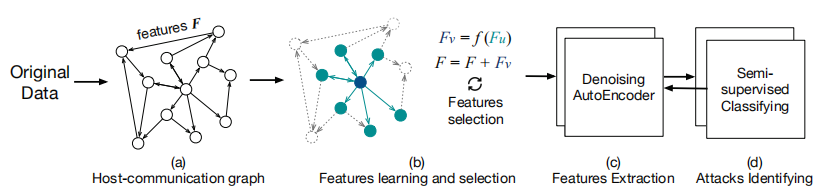
\includegraphics{1.png}}
	\caption{ An overview of the approach architecture.}
	\label{fig}
\end{figure*}

In terms of data preprocessing and fusion, due to the incomplete information of network security data sets and privacy protection policies, the utilization rate of most existing data sets is not high. In the case of existing finite data set, how to improve the prediction efficiency of the model through preprocessing and fusion of finite data is an important research direction.

In terms of model prediction, as the attack activity is obviously less than the normal network activity, the imbalance of data will reduce the accuracy of prediction. Existing learning models can be improved by such methods as semi-supervised classification based on positive and unlabeled data, which is the next topic to be studied.

Therefore, combined with the above two characteristics, the research on information extraction of attackers' attack characteristics in multi-source network security events is not very sufficient. At the same time, there are few studies on the use of multi-source data fusion for attacker feature extraction. Therefore, in this paper, from multi-source network security events, various reference feature extraction methods are used to obtain as many attacker feature patterns as possible, so as to dig out more attackers and predict more attack events.

\section{System Design} \label{model}

The subject of the research is based on a data set, This data set represents 58 consecutive days of de-identified event data collected from five sources within Los Alamos National Laboratory 's corporate internal computer network.It includes four-dimensional network security event information and one-dimensional redteam data, that is, data that has been detected as an attack from the authentication data.

First, the data identified as hazardous events were analyzed to obtain some characteristics. Then, more attack features are extracted from the data by combining the data features of the other four dimensions. Here, some statistical feature extraction, anomaly detection algorithm and graph network construction are used to extract attack features. Feature selection is performed after all extracted attack pattern features are aggregated to determine the final composite feature and customize the structure to describe the attack pattern. Finally, apply the model to the data set to find the undiscovered redteam members. At the same time, in order to verify the accuracy of the model, members that have been defined as redteam can be taken as indicators, and the proportion of tagged redteam members found by the model in the total number can be taken as the observation index of the quality of the feature model. It can also take time as the dimension, and the accuracy of predicting attack events as the index. Finally, because redteam has tagged data only for the first 28 days, it can also use the model to predict attack events for the next days.

The designed model showed in figure 2.

\begin{figure*}[htbp]
	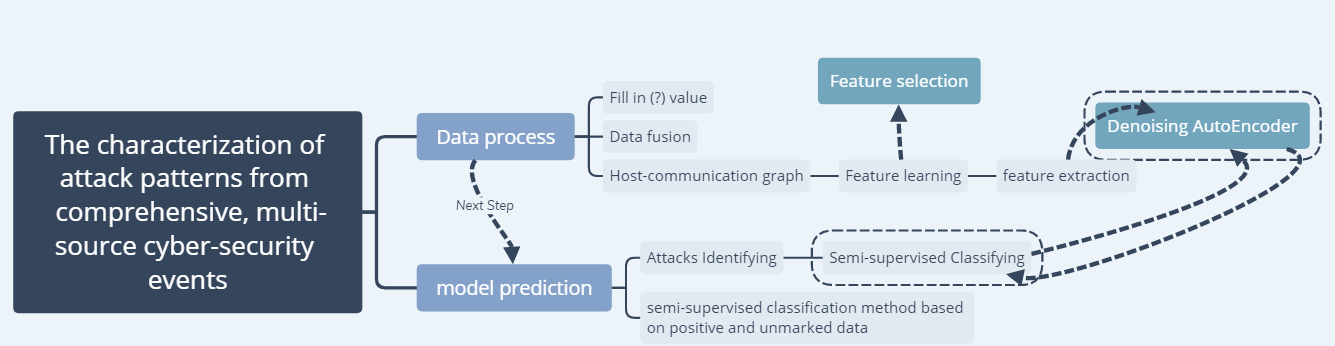
\includegraphics [width=1\textwidth]{2.png}
	\caption{ Model design mind mapping.}
	\label{fig}
\end{figure*}

Based on the data process, we basically have a more perfect algorithm system and structure idea. This section introduces the overall data set preprocessing algorithm, the integration of feature models and the final attack feature model verification ideas and specific implementation strategies.

\subsection{Definition}
Attack event: the attack event includes each record that has been identified as redteam attack event and other characteristics. The attack event is the specific information description of an attack record. The attack event includes network flow, DNS and process-related information records.

Attack pattern: different attack events extracted from attack events have similar characteristics, and these attack events with similar characteristics are combined into one attack pattern. The characteristics of attack events are summarized to obtain specific characteristics description of attack pattern.

Considering that an attack event may have one-dimensional or multidimensional characteristics, this indicates that an attack event has the behavior of a combined attack pattern, that is, the subsequent analysis of attack events based on the combined attack model needs to be considered.

\subsection{DataSet}

The data set mainly contains four - dimensional data and a redteam attack incident file.


\begin{itemize}
	\item Redteam
	\item Authentication Events
	\item Single Computer Process Events
	\item Network Flow Events
	\item Domain Name Service (DNS) Lookup Events
\end{itemize}

This section mainly analyzes the composition of the five data sets and lists the methods and algorithm models for processing each data set. The last four events are mainly combined with Redteam attack event fusion for feature extraction.

\subsubsection{Redteam data set}

The components of redteam events are shown in table 1, including the data that has been detected as an attack from the authentication data. 

\begin{table}[h]
	\caption{Redteam Data Set}
	\vspace{1pt}
	\centering
	\begin{tabular}{p{2.5cm}p{5cm}}
		\hline
		Name & Description \\
		\hline
		time  & The start time of the event\\
		user@domain  & User name and use domain name\\ 
		source computer  & The computer that initiates the authentication\\ 
		destination computer  & The computer that receives the authentication\\
		\hline       
	\end{tabular}
	\label{bs2}
\end{table}

The characteristics of some attackers are extracted from redteam file, such as the most active attackers, the most frequently attacked objects, and the active time distribution of attackers. These attack characteristics can be directly obtained by statistical methods.



\subsubsection{Authentication Events data set}

Authentication events are mostly normal service request data representing an authentication event at the given time, and only a small part of the data is data with attack events. Redteam data is extracted from the authentication data. 
 

\begin{table}[h]
	\caption{Authentication Events Data Set}
	\vspace{1pt}
	\centering
	\begin{tabular}{p{2.5cm}p{5cm}}
		\hline
		Name & Description \\
		\hline
		time  & The start time of the event\\
		source user@domain  & Source user name and use domain name\\ 
		destination user@domain  & Destination user name and use domain name\\ 
		source computer  & The computer that initiates the authentication\\ 
		destination computer  & The computer that receives the authentication\\
		authentication type  & The content of the request sent\\ 
		logon type  & The logon type source computer request\\ 
		authentication orientation  & The authentication request\\ 
		success/failure  & Authentication result\\ 
		\hline       
	\end{tabular}
	\label{bs2}
\end{table}

Therefore, by integrating the two data of redteam data and authentication data, it is only necessary to extract the authentication information containing the attack event in the authentication data to form several attack characteristics.

\subsubsection{Single Computer Process Events data set}

Process files contain process information on a single computer or server.


\begin{table}[h]
	\caption{Single Computer Process Events Data Set}
	\vspace{1pt}
	\centering
	\begin{tabular}{p{2.5cm}p{5cm}}
		\hline
		Name & Description \\
		\hline
		time  & The start time of the event\\
		user@domain  & User name and use domain name\\  
		computer  & The computer that run the process\\ 
		process name  & The running process name\\
		start/end  & The state of the process\\ 
		\hline       
	\end{tabular}
	\label{bs2}
\end{table}

After combining with the redteam file, you can find out the computer or server that is often attacked, monitor the change of process status during the time when the attack is initiated, and find out the process number and process execution time commonly used by the attacker. 

\subsubsection{Network Flow Events data set}

Network flow events represent network flow events collected from a central router within the network.

\begin{table}[h]
	\caption{Network Flow Events Data Set}
	\vspace{1pt}
	\centering
	\begin{tabular}{p{2.5cm}p{5cm}}
		\hline
		Name & Description \\
		\hline
		time  & The start time of the event\\
		duration  & Time the event last\\  
		source computer  & The device that initiated the event\\
		source port  & The port used by the source computer\\
		destination computer  & The computer that receives the event\\
		destination port  & The port used by the destination computer\\
		protocol  & The protocol number\\ 
		packet count  & The number of packets during the event\\
		byte count  & The number of bytes during the event\\ 
		\hline       
	\end{tabular}
	\label{bs2}
\end{table}

By analyzing the network stream characteristics related to the attacker in redteam, the port number commonly used by the attacker, the protocol used by the attacker, packet sent and bytes number can be found as the characteristics. From the time dimension, the network flow state near the attack period can be found out as the attack characteristic.

Because most of the data in the network stream data are normal data, and only a small part are possible attack events, abnormal detection algorithm can also be applied in the data stream data set to detect abnormal data and find out the attack characteristics.

\subsubsection{Domain Name Service (DNS) Lookup Events}

DNS data represents the domain name service (DNS) lookup event collected from a central DNS server in the network, displays the DNS lookup of the source computer against the resolved computer at a given time, and represents a possible network connection from the source computer to the target computer.

\begin{table}[h]
	\caption{Domain Name Service (DNS) Lookup Events Set}
	\vspace{1pt}
	\centering
	\begin{tabular}{p{2.5cm}p{5cm}}
		\hline
		Name & Description \\
		\hline
		time  & The start time of the event\\
		source computer  & The device that initiated the event\\
		computer resolved  & The computer or server being parsed\\
		\hline       
	\end{tabular}
	\label{bs2}
\end{table}

According to the domain name service lookup information, the number of domain name service requests initiated by the attacker and the relationship between the time period can be obtained to obtain the attack characteristics.

\subsection{Single Feature Extraction}

Model based on the statistical characteristics of the feature extraction, the characteristics of the attacker was formed by simple encoding attack feature vector, the characteristics of these attacks has find the attacker's can discuss, but these features may be related to the actual attacker behavior has certain discrepancy, so from time and space dimensions anticipation on the attacker's behavior.

\subsubsection{Redteam Dataset processing}
The first is the separate processing of redteam file, which processes all attack events and extracts the attack object of each attacker and the attack times of each attack object. It can be found from the data that there are only four attack initiators among the detected attack events, among which the attack frequency from C17693 is as much as 701, while the attack frequency of other attackers is relatively less. The attack frequency distribution of attackers is shown in figure 3.

\begin{figure}[htpb]
	\centering
	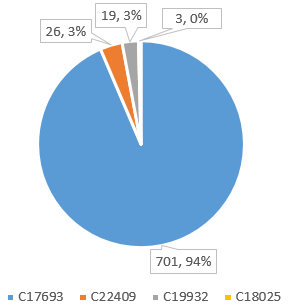
\includegraphics []{3.png}
	\caption{Attack frequency and attacker source distribution1}
	\label{fig}
\end{figure}



Second, most victims suffered only one attack, and some were the main targets. Different attackers have different targets. 

Attack events are numbered from 1 and the sequence of attack events is marked for subsequent processing. The graph below shows the distribution diagram of the number of attack events. The abscissa of the bar graph represents the attacker, and the ordinate represents the number of attacks of the attacked with different colors. The total length of the ordinate represents the total number of attacks, and different colors represent different attacked objects.

\begin{figure}[htpb]
	\centering
	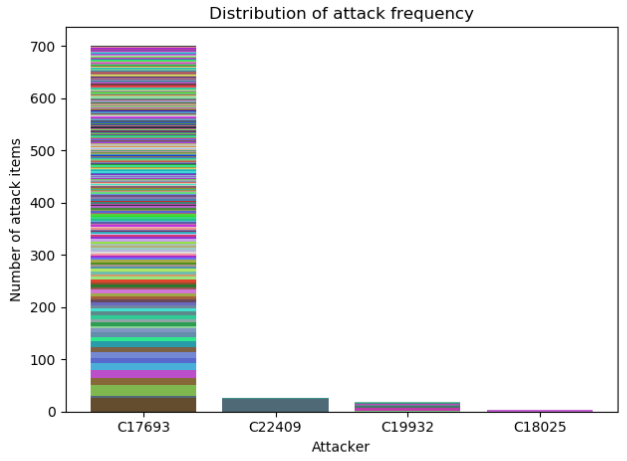
\includegraphics []{6.png}
	\caption{Attack frequency and attacker source distribution2}
	\label{fig}
\end{figure}

\subsubsection{Single Computer Process Events Dataset processing}

Process Numbers are coded to count the process Numbers of each attack event and the number of occurrences in that attack. So each attack event is represented by a vector that has several elements of the process. Obviously, the degree of clustering of high-dimensional data cannot be controlled manually, nor can a good visualization be formed. Therefore, a high-dimensional data dimensionality reduction algorithm is referred to here for dimensionality reduction processing of high-dimensional characteristic data of each attack event. The characterization of each attack event becomes a two-dimensional vector.

The t-sne method was proposed by Hinton et al. T-sne USES the t-distribution with heavier and longer tail distribution in low dimensional space to avoid crowding and optimization problems. T-sne converts the similarity between data points into conditional probability. The similarity of data points in the original space is represented by gaussian joint distribution, and the similarity of data points in embedded space is represented by student t distribution. The KL divergence of the joint probability distribution of the original space and the embedded space (an index used to evaluate the similarity of the two distributions) is used to evaluate the embedding effect. The function of KL divergence is taken as the loss function, and the loss function is minimized through the gradient descent algorithm, and finally the convergence result is obtained.

\begin{figure}[htpb]
	\centering
	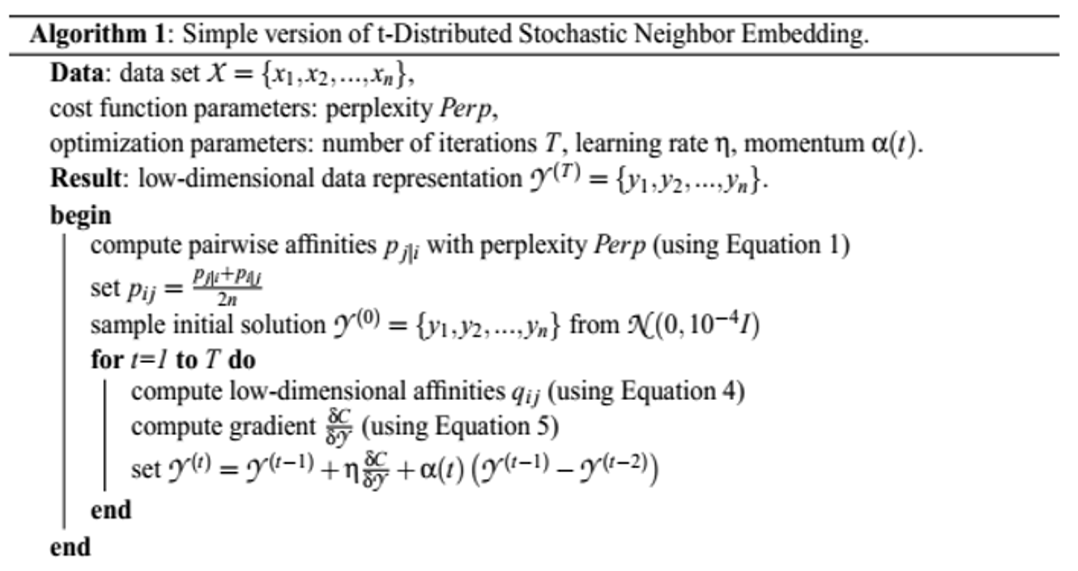
\includegraphics [width=1\textwidth]{7.png}
	\caption{t-SNE pseudocode}
	\label{fig}
\end{figure}

Through the algorithm, the data format obtained is [attack event encoding, dimensionality reduction feature 1, dimensionality reduction feature 2]. Since the feature is reduced to 2d, it can be visualized (figure 6).

\begin{figure}[htpb]
	\centering
	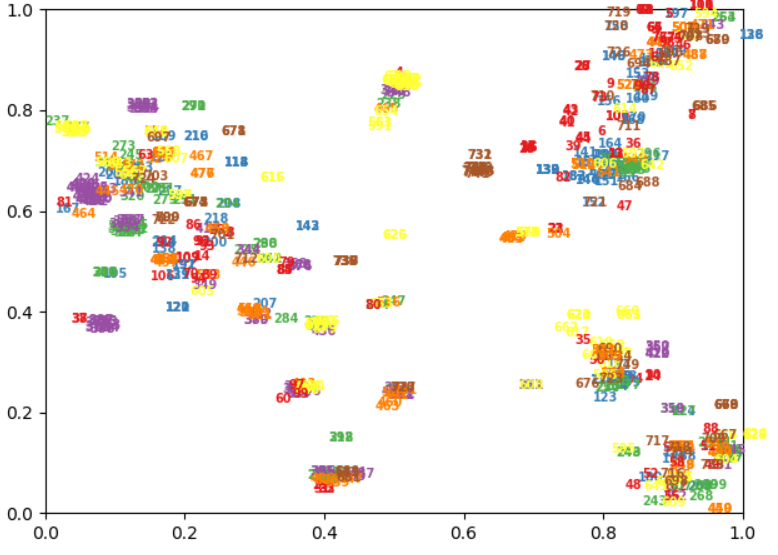
\includegraphics [width=1\textwidth]{proc.png}
	\caption{reduction feature of process events distribution}
	\label{fig}
\end{figure}

Gaussian mixture model, or GMM. Gaussian mixture model is the accurate quantization of things with gaussian probability density function, which decomposes a thing into several models based on the travel of gaussian probability density function. The curve and mathematical expression are used to approximate the simulated classification scatter graph, that is, the characteristic scatter distribution. Gaussian mixture curve is superimposed by several single gaussian functions. By solving multiple single gaussian models, and fusing multiple single gaussian models into one model through certain weights, it is the final gaussian mixture model.



The algorithm of GMM is as follows:

\begin{itemize}
	\item For each sample point $i$, calculate the probability that it is generated by a different component (the $k$th component) \\
	$r(i,k)=\frac{\pi_{k}N(x_{i}|\mu_{k},\sigma_{k})}{\sum_{j=1}^{K}\pi_{j}N(x_{i}|\mu_{j},\sigma_{j})}$
	
	\item Step2: update the parameters $\pi_{i}$, $\mu_{i}$ and $\sigma_{i}$ by $r(i,k)$ of each sample point
	\item Step3: return to Step1 and update iteratively
\end{itemize}

Process classification results are obtained by clustering algorithm. There are eight types of processes, that is, eight attack patterns on the process side. Stores a two-dimensional eigenvector value as a characteristic representation of each attack pattern. The following figure shows eight clusters formed after GMM clustering, representing eight attack modes.

\begin{figure}[htpb]
	\centering
	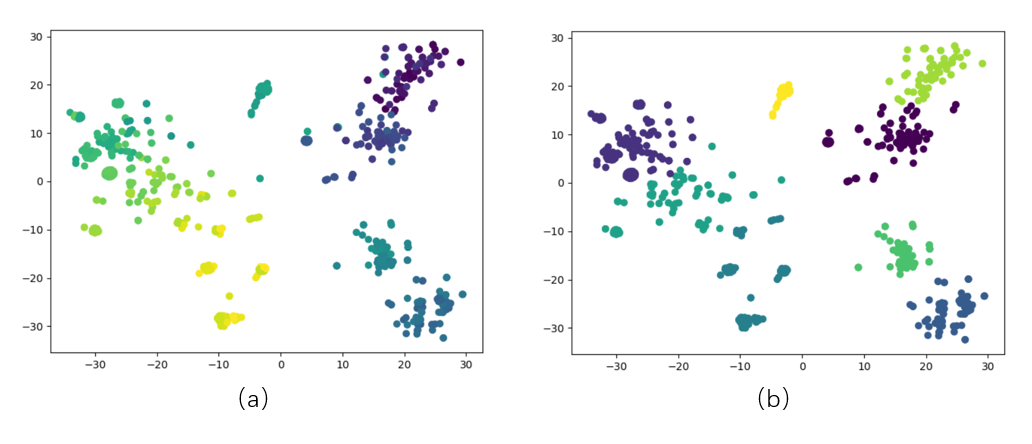
\includegraphics [width=1\textwidth]{8.png}
	\caption{Brich clustering(a),GMM clustering results - Eight attack patterns(b)}
	\label{fig}
\end{figure}

Previously, Birch Algorithm (balanced iterative specification and clustering using a hierarchical approach) was used. It is to form a clustering feature tree through clustering feature (CF), and the number of CF in root layer is the number of clustering. Clustering feature (CF) : each CF is a triple, which can be represented by (N, LS, SS), where N represents the number of sample points in this CF; LS represents the sum of the eigendimensions of the sample points in CF, and SS represents the sum of the squares of the eigendimensions of the sample points in CF.

This algorithm can display the clustering results without defining the classification quantity. From the comparison diagram of the two algorithms, it can be seen that GMM algorithm is better than Brich algorithm, so GMM clustering algorithm is finally adopted for feature extraction.

\subsubsection{DNS Dataset processing}
DNS service mainly includes the domain name service request from the source computer to the target computer. It can be seen from the request that the attacker extracts the attack characteristics of whether there are frequent domain name service requests near the attack event period.

One important piece of information you get from the redteam file is information marked as an attacker. At the same time also by the attacker computer code information, find out the attacker from DNS file request to the victims of the domain name service, all the related domain names containing all of the time online request, mainly focused on the domain name service request number and the attacker and the possibility attacked by the attacker's number and attack relationship analysis. Call pyhon's native networkx library to build a directed graph for visualization.

Here originally want to build all DNS request information with different colors to distinguish possible normal request and attack, but the DNS file is too large, a graph structure is very complex and not clear, so the only mark the attacker and the attacker's way to visualize the attacker to be the attacker's DNS request times change.

The DNS frequency distribution of attackers and victims is shown in figure 4.

\begin{figure}[htpb]
	\centering
	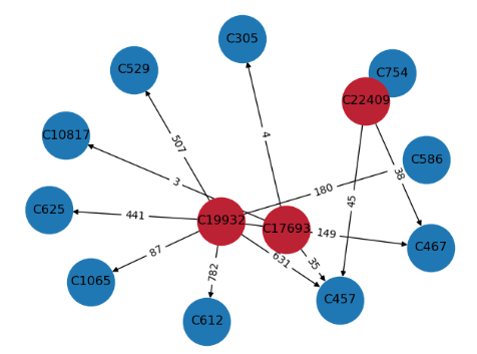
\includegraphics [width=7cm]{4.png}
	\caption{Attack events and DNS request times}
	\label{fig}
\end{figure}

In the figure, the red is the attacker and the blue is the target. The weight on the edge of the directed graph represents the number of DNS domain name service requests made by the attacker to the target.

For example, the figure below shows the number of attacks made by an attacker against the attacked.

\begin{figure}[htpb]
	\centering
	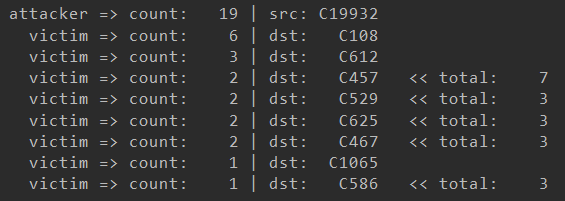
\includegraphics [width=9cm]{5.png}
	\caption{A certain attacker attack information statistics}
	\label{fig}
\end{figure}

It can be seen from the information in the figure that C612, C457, C625 and C1029 are all the objects frequently requested for DNS domain name service, and they are also the main objects attacked by C19932. Therefore, it can be concluded that the attacker will make multiple DNS service requests to the attacker to achieve its attack purpose, which can be regarded as an attack characteristic.

So getting DNS request information (with/without or in quantity) can be used as a basis for an attack pattern. Given the attack time interval, the DNS request information within 2 days of the control time is the valid information associated with the attack event.

However, the extracted data results are not very obvious, and DNS data can only be analyzed as auxiliary data to determine an attack pattern. Of the four attackers identified in the redteam file, only two attackers' DNS requests were captured, and only four attack events' DNS requests could be captured. The specific data is as follows.

The attacker C17693 has only one DNS event catched.

\begin{table}[h]
	\caption{DNS events associsted with C17693 attacking C10817}
	\vspace{1pt}
	\centering
	\begin{tabular}{p{2.5cm}p{2.5cm}p{2.5cm}p{2.5cm}}
		\hline
		Attack No. & Timestamp & Src C. & Dst C. \\
		\hline
		698 & 2300048 & C17693 & C10817\\
		698 & 2300049 & C17693 & C10817\\
		\hline       
	\end{tabular}
	\label{bs2}
\end{table}

Based on the network flow events discussed below, it can be seen that the attack mode of C17693 mainly focuses on the network flow and process characteristics, so DNS has very few attack features, but it can also be used as an attack mode different from other attack modes. At the same time, the attacked C10817 does not appear in the network stream data feature, so DNS feature may be the difference that describes its feature.

The attacker C19933 has three DNS events catched. 
The attack time of the three data is also similar, so it can be concluded that some attackers often attack different computer hosts several times at a certain time. The following is the DNS record related to the attack event of C19932.

\begin{table}[h]
	\caption{DNS events associsted with C19932 attacking C457}
	\vspace{1pt}
	\centering
	\begin{tabular}{p{2.5cm}p{2.5cm}p{2.5cm}p{2.5cm}}
		\hline
		Attack No. & Timestamp & Src C. & Dst C. \\
		\hline
		733 & 2471396 & C19932 & C457\\
		733 & 2471480 & C19932 & C457\\
		733 & 2477358 & C19932 & C457\\
		733 & 2483481 & C19932 & C457\\
		733 & 2486959 & C19932 & C457\\
		733 & 2539627 & C19932 & C457\\
		733 & 2539631 & C19932 & C457\\
		733 & 2539679 & C19932 & C457\\
		733 & 2540555 & C19932 & C457\\
		733 & 2541455 & C19932 & C457\\
		733 & 2542355 & C19932 & C457\\
		733 & 2543255 & C19932 & C457\\
		733 & 2544155 & C19932 & C457\\
		733 & 2545055 & C19932 & C457\\
		733 & 2546855 & C19932 & C457\\
		733 & 2547755 & C19932 & C457\\
		733 & 2548655 & C19932 & C457\\
		733 & 2550455 & C19932 & C457\\
		733 & 2552256 & C19932 & C457\\
		\hline       
	\end{tabular}
	\label{bs2}
\end{table}

By observing the above DNS access records, it can be found that some attack mode will continuously send DNS requests to the target computer frequently for a long time. This attack mode is more likely to cause denial of service attacks, which can be used as an auxiliary description feature of an attack mode.

\begin{table}[h]
	\caption{DNS events associsted with C19932 attacking C529}
	\vspace{1pt}
	\centering
	\begin{tabular}{p{2.5cm}p{2.5cm}p{2.5cm}p{2.5cm}}
		\hline
		Attack No. & Timestamp & Src C. & Dst C. \\
		\hline
		730 & 2377419 & C19932 & C529\\
		730 & 2377433 & C19932 & C529\\
		730 & 2377561 & C19932 & C529\\
		730 & 2387721 & C19932 & C529\\
		\hline       
	\end{tabular}
	\label{bs2}
\end{table}

\begin{table}[h]
	\caption{DNS events associsted with C19932 attacking C625}
	\vspace{1pt}
	\centering
	\begin{tabular}{p{2.5cm}p{2.5cm}p{2.5cm}p{2.5cm}}
		\hline
		Attack No. & Timestamp & Src C. & Dst C. \\
		\hline
		734 & 2471503 & C19932 & C625\\
		\hline       
	\end{tabular}
	\label{bs2}
\end{table}

Most of the network flow data is normal network data flow, but only a small part of the network flow data as abnormal, these data may often become an important indicator of the attack by attackers. 

Therefore, the anomaly detection algorithm is adopted to detect the abnormal part of the network stream data. There are many kinds of anomaly detection algorithms, and the one that is more suitable for network flow data detection is the isolated forest algorithm. 

The isolated forest algorithm is based on the partition idea. The idea is that if a random hyperplane is used to split data space, two subspaces can be generated at one time. And then continue to cut each subspace with a random hyperplane, and keep going until there is only one data point in each subspace. Intuitively, clusters with high density can be cut many times before they stop cutting, but those with low density can easily end up in a subspace very early. Therefore, it is easy to find the low-density points as outliers, that is, abnormal data in the network flow. Its pseudocode is as follows.

\begin{algorithm}[h]  
	\caption{iTree(X,e,h)}  
	\begin{algorithmic}[1] 
		\Require  
		X - input data;  
		e - current height;  
		h - height limit;  
		\Ensure  
		an iTree; 
		\If{$e \geq h$ OR $|X| \leq 1$ }  
		\Return $exNode{Size \leftarrow |X|}$;
		\Else
		\State $Randomly$ $select$ $an$ $attribute$ $q$;
		\State $Randomly$ $select$ $a$ $split$ $point$ $p$ $between$ $min$ $and$ $max$ $values$ $of$ $attribute$ $q$ $in$ $X$;
		\State $X_l$ $\leftarrow$ $filter(X,q < p)$ $,$ $X_r$ $\leftarrow$ $filter(X,q \geq p)$;
		\State	
		\Return $inNode{Left \leftarrow iTree(X_l,e+1,h)}$;	
		\State		
		\Return	$inNode{Right \leftarrow iTree(X_r,e+1,h)}$	;
		\State	
		\Return $inNode{SplitAttr \leftarrow q,SplitValue \leftarrow p}$;
		\EndIf 
		\label{code:recentEnd}  
	\end{algorithmic}  
\end{algorithm}  

The abnormal DNS events obtained from the operation include the DNS characteristics of the above four attack events. However, due to many chaotic factors, there are many abnormal DNS data determined by the isolated forest algorithm, and its correctness cannot be verified.

\subsubsection{Network Flow Events Dataset processing}
Obtain the network flow information of each attacker (a total of four) and its corresponding victim, and find out the network flow information around the time of the attack event (obtain the attacker's customary port number and the victim port number).

Network flow information mainly consists of the following components [duration, source port, target port, protocol, packet count, byte count]. Through observation, duration, protocol, packet count, byte count are basically the same, but the changes of these characteristics are not very obvious in different attack events. Therefore, the analysis data will be focused on the characteristics of the port number.

The port number is numbered and the number of times of use of the port is taken as its feature, forming a multi-dimensional feature vector. T-sne dimensionality reduction processing was conducted on the data in the same way as process data processing, and the result diagram was obtained through GMM clustering as follows:

\begin{figure}[htpb]
	\centering
	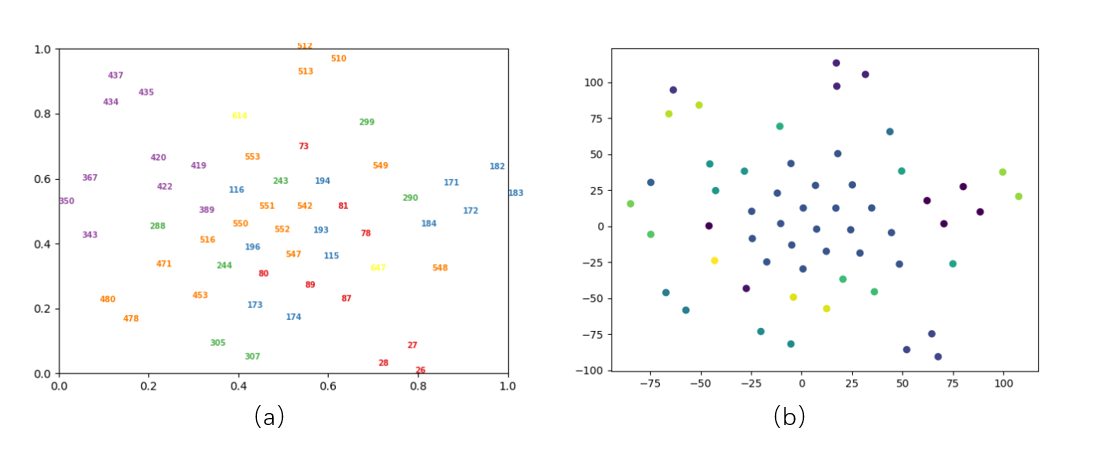
\includegraphics [width=1\textwidth]{9.png}
	\caption{port distribution(a),GMM clustering results - None features(b)}
	\label{fig}
\end{figure}

As can be seen from the figure, the data distribution does not have a fixed shape, so each port number is independent, that is, the port number distribution has no special characteristics. If the number of visits on a fixed port exceeds a certain threshold, it may be used as a basis for the attack mode. Therefore, the access data set of each port is counted, and the threshold is calculated. If the threshold is exceeded, it can be determined as an attack event.

\begin{figure}[htpb]
	\centering
	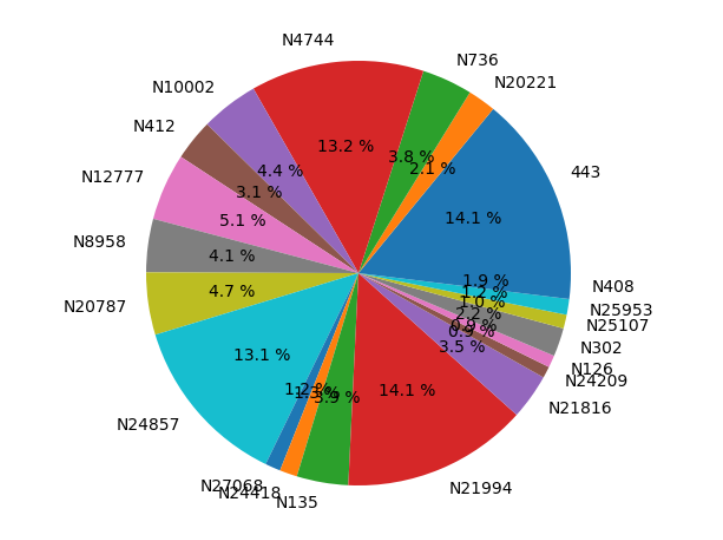
\includegraphics [width=1\textwidth]{10.png}
	\caption{port distribution}
	\label{fig}
\end{figure}

The port number is recorded for subsequent feature matching operations.


\subsubsection{Authentication Events Dataset processing}
Extract redteam specific data to obtain authentication type[at], logon type[lt], authentication orientation[ao], [success/failure]). Obtain the specific data of each attack event, and after comparison, it is found that the last three key information contains all the same data. Meanwhile, the last bit of data is mostly success, with only a few dozen records as failures.

The last four bits of information are only in two forms and are represented as follows:

\begin{table}[h]
	\caption{Authentication Events Form of attack events}
	\vspace{1pt}
	\centering
	\begin{tabular}{p{3cm}p{3cm}p{4cm}p{3cm}}
		\hline
		authentication type & logon type & authentication orientation & Success/Fail \\
		\hline
		NTLM & Network & LogOn & Success\\
		NTLM & Network & LogOn & Fail\\
		\hline       
	\end{tabular}
	\label{bs2}
\end{table}


\subsection{Combined Feature Extraction}
In addition to attack events with a single feature, there are also attack events that combine attack patterns in three directions, which is called combinatorial attack.

\subsubsection{Process combined with DNS}
Since DNS data is less, the association between DNS and process information can be directly analyzed. Through simple search, it can be found that both attack event 733 and attack event 698 belong to attack mode 2. The DNS information associated with both attacks is frequently and continuously accessed. Combined with the knowledge of relevant denial-of-service attacks, the characteristics of this attack pattern can be linked to the actual attack model. So 733 and 689 attacks can be called combined mode attacks.

However, the attack events 730 and 734 have no process information, so they only contain one or two short DNS requests. The characteristics of such attack events are difficult to describe, because only DNS requests exist, so there is no extra information for specific classification.


\section{Evaluation and Discussion}
Since the characteristics of the three dimensions are mainly analyzed, the attack events are found from the source data according to the characteristics of the attack model of the three dimensions. Because the source data was too large (over 100 GB), I extracted the data of day 8 from it for test analysis.

\subsection{Process}
Process events from the eighth day, every hour to extract different host process information, the process information and processes the format of the data processing, is a multidimensional data, will be the same dimension, the multi-dimensional data with the eight kinds of feature model compare (threshold can be adjusted, chose the highest accuracy threshold).

After the data is sorted, the events that might contain the process data are identified from the authentication data based on the data information. These events also satisfy the authentication characteristics of the attack event. After these layers of filtering, the rest of the data is likely to become an attack event data.

By comparing the predicted attack events with the total attack events on the eighth day, a total of 30 data points were successfully compared.

This is only a one-dimensional feature comparison, and the total accuracy ratio needs to be analyzed after network flow events are processed.

At the same time, the analysis of the process information also found a lot of data that was not on the redteam list for possible attacks, including some that had never been seen before, and also many hosts that were frequently targeted. 

\subsection{Flows}
First, the common port number of attackers is obtained from the feature extraction model:

443, N20221 N736 N4744, N10002, N412, N12777, N8958, N20787, N24857, N27068, N24418, N135, N21994, N21816, N24209, N126, N302, N25107, N25953, N408

Extract packages (that is, network flow information) from different hosts every hour from the network flow event on the eighth day. Statistics the occurrence of events sent from the above port and records their specific data.

Extract at least ten data sent from each port as objects initially suspected of being attacked. Combining with the authentication data, the suspected objects of these attack events are extracted from the authentication data, and the authentication information that may become attack events is obtained by filtering according to the characteristics of the authentication events.

\begin{figure}[htpb]
	\centering
	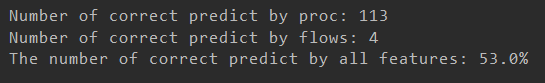
\includegraphics [width=0.5\textwidth]{12.png}
	\caption{port distribution}
	\label{fig}
\end{figure}

A total of 117 marked attack events were extracted from proc data and flow data, with a total of 222 attack events, and the accuracy of the algorithm was 53.0\%

\subsection{DNS}
Dns requests have a hard time finding the identity of the attacker, but hosts that are frequently attacked are bound to receive many Dns requests. So the eighth day of DNS request statistics, can find out the frequently attacked objects.

In redteam attack event, 173 victims were included. DNS request data was analyzed and filtered, and 41 victims were found to be attacked objects in redteam attack event.
\begin{figure}[htpb]
	\centering
	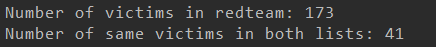
\includegraphics [width=0.5\textwidth]{11.png}
	\caption{dns finding victims}
	\label{fig}
\end{figure}

\begin{figure}[htpb]
	\centering
	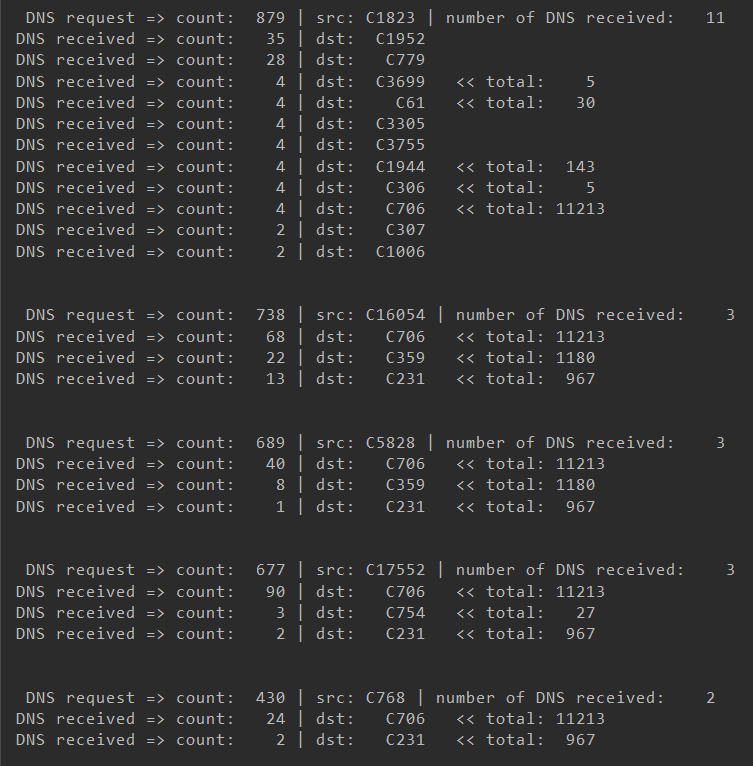
\includegraphics [width=0.7\textwidth]{13.png}
	\caption{unmarked attackers}
	\label{fig}
\end{figure}



List of attack objects:

C92 C1823, C1611 C1089, C12682, C2597, C11039, C307, C1006, C3173, C2057, C2519, C1028, C492, C3305, C3755, C306, C3699, C464, C1710, C1549, C742, C1183, C1503, C801, C2091, C798, C395, C754, C779, C61, C1797, C46, C1952, C1732, C101 5, C1944, C2079, C231 C359, C706


\section{Conclusion and future work}
In this paper, feature extraction, dimension reduction, hierarchical clustering and other methods are used to analyze the event data of a four-dimensional multi-source network. Finally, four attack features in different directions were extracted from the four-dimensional data, including 11 attack modes and 1 combined attack modes. Finally, the detection accuracy of the attack event reached 53\%. It also discovered more potential attack data and potential attackers that were not marked as attack events.

The measures in this paper are helpful for extracting and analyzing potential dangerous events from multi-source network security incidents. It also has certain adaptability to data perturbation and data deletion in various directions. From the spatial dimension, we can grasp the relationship between the attacker and the attacked well, and discover more attackers and attack events through this connection.

However, from the perspective of time dimension, this model does not grasp the information of time dimension well. The analysis of the characteristics only briefly summarizes a certain range of time, but the analysis of the specific time dimension, including the interval between attacks of a certain attacker, which can be used as a feature, is not covered.

The future research can focus on the analysis of the attacker, the description of the attacker's behavior and the change of the attacker's attack in the time dimension. Due to limited computer resources, it is impossible to construct a large network diagram to visually show the network connection between the attacker and the attacked. If we can construct a complete network structure diagram or host communication diagram, it may be more helpful for feature extraction.

\begin{thebibliography}{99}  
	\bibitem{ref1}M. Chen, Y. Yao, J. Liu, B. Jiang, L. Su and Z. Lu, "A Novel Approach for Identifying Lateral Movement Attacks Based on Network Embedding," 2018 IEEE Intl Conf on Parallel \& Distributed Processing with Applications, Ubiquitous Computing \& Communications, Big Data \& Cloud Computing, Social Computing \& Networking, Sustainable Computing \& Communications (ISPA/IUCC/BDCloud/SocialCom/SustainCom), Melbourne, Australia, 2018, pp. 708-715.
	doi: 10.1109/BDCloud.2018.00107  
	\bibitem{ref2}J. Hogan and N. M. Adams, "A Study of Data Fusion for Predicting Novel Activity in Enterprise Cyber-Security," 2018 IEEE International Conference on Intelligence and Security Informatics (ISI), Miami, FL, 2018, pp. 37-42.
	doi: 10.1109/ISI.2018.8587400  
	\bibitem{ref3}H. Djidjev G. Sandine C. Storlie S. Vander Wiel "Graph based statistical analysis of network traffic" Proceedings of the Ninth Workshop on Mining and Learning with Graphs (MLG) 2011. 
	\bibitem{ref4}L. Breiman "Random forests" Machine learning vol. 45 no. 1 pp. 5-32 2001.
	\bibitem{ref5}A. Oprea Z. Li T.F. Yen S.H. Chin S. Alrwais "Detection of early-stage enterprise infection by mining large-scale log data" 2015 45th Annual IEEE/IFIP International Conference on Dependable Systems and Networks pp. 45-56 June 2015.
	\bibitem{ref6}R. Zhao and K. Mao, "Semi-Random Projection for Dimensionality Reduction and Extreme Learning Machine in High-Dimensional Space," in IEEE Computational Intelligence Magazine, vol. 10, no. 3, pp. 30-41, Aug. 2015.
	doi: 10.1109/MCI.2015.2437316
	\bibitem{ref7}A. Ben Ayed, M. Ben Halima and A. M. Alimi, "Adaptive fuzzy exponent cluster ensemble system based feature selection and spectral clustering," 2017 IEEE International Conference on Fuzzy Systems (FUZZ-IEEE), Naples, 2017, pp. 1-6.
	doi: 10.1109/FUZZ-IEEE.2017.8015721

	
\end{thebibliography}



\end{document}